\documentclass{vkr}
\usepackage[english, russian]{babel} % переносы
\usepackage{graphicx} % для вставки картинок
\graphicspath{{images/}} % путь к изображениям
\usepackage[hidelinks]{hyperref}
\usepackage{float} % определяет метод H для рисунка с переносом на следующую страницу, ели не помещается
\usepackage{pdflscape}
\addto{\captionsrussian}{\renewcommand{\refname}{СПИСОК ИСПОЛЬЗОВАННЫХ ИСТОЧНИКОВ}}
\usepackage{xltabular} % для вставки таблиц
\usepackage{makecell}
\renewcommand\theadfont{} % шрифт в /thead
\usepackage{array} % для определения новых типов столбцов таблиц
\newcolumntype{T}{>{\centering\arraybackslash}X} % новый тип столбца T - автоматическая ширина столбца с выравниванием по центру
\newcolumntype{R}{>{\raggedleft\arraybackslash}X} % новый тип столбца R - автоматическая ширина столбца с выравниванием по правому краю
\newcolumntype{C}[1]{>{\centering\let\newline\\\arraybackslash\hspace{0pt}}m{#1}} % новый тип столбца C - фиксированная ширина столбца с выравниванием по центру
\newcolumntype{r}[1]{>{\raggedleft\arraybackslash}p{#1}} % новый тип столбца r - фиксированная ширина столбца с выравниванием по правому краю
\newcommand{\centrow}{\centering\arraybackslash} % командой \centrow можно центрировать одну ячейку (заголовок) в столбце типа X или p, оставив в оcтальных ячейках другой тип выравнивания
\newcommand{\finishhead}{\endhead\hline\endlastfoot}
\newcommand{\continuecaption}[1]{\captionsetup{labelformat=empty} \caption[]{#1}\\ \hline }
\usepackage{etoolbox}
\AtBeginEnvironment{xltabular}{\refstepcounter{tablecnt}} % подсчет таблиц xltabular, обычные таблицы подсчитываются в классе

\usepackage[tableposition=top]{caption} % подпись таблицы вверху
\captionsetup{strut=off}
\setlength{\intextsep}{0pt} % Vertical space above & below [h] floats
\setlength{\textfloatsep}{0pt} % Vertical space below (above) [t] ([b]) floats
\DeclareCaptionLabelFormat{gostfigure}{Рисунок #2} %подпись рисунка
\DeclareCaptionLabelFormat{gosttable}{Таблица #2} %подпись таблицы
\DeclareCaptionLabelSeparator{gost}{~--~} %разделитель в рисунках и таблицах
\captionsetup{labelsep=gost}
\captionsetup[figure]{aboveskip=10pt,belowskip=4mm,justification=centering,labelformat=gostfigure} % настройка подписи рисунка
\captionsetup[table]{font={stretch=1.41},skip=0pt,belowskip=0pt,aboveskip=8.5pt,singlelinecheck=off,labelformat=gosttable} % настройка подписи таблицы

\setlength{\LTpre}{8mm} % отступ сверху таблицы
\setlength{\LTpost}{6mm} % отступ снизу таблицы

\usepackage{enumitem}
\setlist{nolistsep,wide=\parindent,itemindent=*} % отступы вокруг списков, выравнивание с учетом разделителя

\usepackage{enumitem}
\renewcommand{\labelitemi}{\textbullet}

\usepackage{color} %% это для отображения цвета в коде
\usepackage{listings} %% листинги кода
\setmonofont[Scale=0.7]{Verdana} % моноширный шрифт для листинга

\definecolor{codegreen}{rgb}{0,0.6,0}
\definecolor{codegray}{rgb}{0.5,0.5,0.5}
\definecolor{codepurple}{rgb}{0.58,0,0.82}

\lstset{ %
language=C,                 % выбор языка для подсветки (здесь это С)
numbers=left,               % где поставить нумерацию строк (слева\справа)
numberstyle=\tiny,           % размер шрифта для номеров строк
stepnumber=1,                   % размер шага между двумя номерами строк
numbersep=5pt,                % как далеко отстоят номера строк от подсвечиваемого кода
commentstyle=\color{codegreen},
keywordstyle=\color{magenta},
numberstyle=\tiny\color{codegray},
stringstyle=\color{codepurple},
basicstyle=\linespread{0.95}\ttfamily,
backgroundcolor=\color{white}, % цвет фона подсветки - используем \usepackage{color}
showspaces=false,            % показывать или нет пробелы специальными отступами
showstringspaces=false,      % показывать или нет пробелы в строках
showtabs=false,             % показывать или нет табуляцию в строках
frame=single,              % рисовать рамку вокруг кода
tabsize=2,                 % размер табуляции по умолчанию равен 2 пробелам
captionpos=t,              % позиция заголовка вверху [t] или внизу [b] 
breaklines=true,           % автоматически переносить строки (да\нет)
breakatwhitespace=false, % переносить строки только если есть пробел
escapeinside={\%*}{*)}   % если нужно добавить комментарии в коде
}

\makeatletter % чтобы допускались русские комментарии в листингах
\lst@InputCatcodes
\def\lst@DefEC{%
 \lst@CCECUse \lst@ProcessLetter
  ^^80^^81^^82^^83^^84^^85^^86^^87^^88^^89^^8a^^8b^^8c^^8d^^8e^^8f%
  ^^90^^91^^92^^93^^94^^95^^96^^97^^98^^99^^9a^^9b^^9c^^9d^^9e^^9f%
  ^^a0^^a1^^a2^^a3^^a4^^a5^^a6^^a7^^a8^^a9^^aa^^ab^^ac^^ad^^ae^^af%
  ^^b0^^b1^^b2^^b3^^b4^^b5^^b6^^b7^^b8^^b9^^ba^^bb^^bc^^bd^^be^^bf%
  ^^c0^^c1^^c2^^c3^^c4^^c5^^c6^^c7^^c8^^c9^^ca^^cb^^cc^^cd^^ce^^cf%
  ^^d0^^d1^^d2^^d3^^d4^^d5^^d6^^d7^^d8^^d9^^da^^db^^dc^^dd^^de^^df%
  ^^e0^^e1^^e2^^e3^^e4^^e5^^e6^^e7^^e8^^e9^^ea^^eb^^ec^^ed^^ee^^ef%
  ^^f0^^f1^^f2^^f3^^f4^^f5^^f6^^f7^^f8^^f9^^fa^^fb^^fc^^fd^^fe^^ff%
  ^^^^20ac^^^^0153^^^^0152%
  % Basic Cyrillic alphabet coverage
  ^^^^0410^^^^0411^^^^0412^^^^0413^^^^0414^^^^0415^^^^0416^^^^0417%
  ^^^^0418^^^^0419^^^^041a^^^^041b^^^^041c^^^^041d^^^^041e^^^^041f%
  ^^^^0420^^^^0421^^^^0422^^^^0423^^^^0424^^^^0425^^^^0426^^^^0427%
  ^^^^0428^^^^0429^^^^042a^^^^042b^^^^042c^^^^042d^^^^042e^^^^042f%
  ^^^^0430^^^^0431^^^^0432^^^^0433^^^^0434^^^^0435^^^^0436^^^^0437%
  ^^^^0438^^^^0439^^^^043a^^^^043b^^^^043c^^^^043d^^^^043e^^^^043f%
  ^^^^0440^^^^0441^^^^0442^^^^0443^^^^0444^^^^0445^^^^0446^^^^0447%
  ^^^^0448^^^^0449^^^^044a^^^^044b^^^^044c^^^^044d^^^^044e^^^^044f%
  ^^^^0401^^^^0451%
  %%%
  ^^00}
\lst@RestoreCatcodes
\makeatother


% Режим шаблона (должен быть включен один из трех)
%\ВКРtrue
\Практикаtrue
%\Курсоваяtrue

\newcommand{\Дисциплина}{<<Проектирование и архитектура программных систем>>} % для курсовой
\newcommand{\КодСпециальности}{09.03.04} % Курсовая
\newcommand{\Специальность}{Программная инженерия} % Курсовая
\newcommand{\Тема}{Разработка web-сайта «Русатом – Аддитивные технологии» на платформе} % ВКР Курсовая
\newcommand{\ТемаВтораяСтрока}{1С-Битрикс}
\newcommand{\ГдеПроводитсяПрактика}{ООО «МЦОБ. Онлайн-сервисы»} % для практики
\newcommand{\РуководительПрактПредпр}{Куркина А. В.} % для практики
\newcommand{\ДолжнРуководительПрактПредпр}{директор} % для практики
\newcommand{\РуководительПрактУнивер}{Чаплыгин А. А.} % для практики
\newcommand{\ДолжнРуководительПрактУнивер}{к.т.н. доцент} % для практики
\newcommand{\Автор}{И. И. Иванов}
\newcommand{\АвторРод}{Иванова И.И.}
\newcommand{\АвторПолностьюРод}{Боева Антона Владимировича} % для практики
\newcommand{\Шифр}{хх-хх-хххх}
\newcommand{\Курс}{4 } % для практики
\newcommand{\Группа}{ПО-11б}
\newcommand{\Руководитель}{А. А. Чаплыгин} % для ВКР и курсовой
\newcommand{\Нормоконтроль}{А. А. Чаплыгин} % для ВКР
\newcommand{\ЗавКаф}{А. В. Малышев} % для ВКР
\newcommand{\ДатаПриказа}{«07» апреля 2023~г.} % для ВКР
\newcommand{\НомерПриказа}{1505-с} % для ВКР
\newcommand{\СрокПредоставления}{«13» июня 2023~г.} % для ВКР, курсового

\begin{document}
\maketitle
\ifПрактика{}\else{
   \newpage
\begin{center}
\large\textbf{Минобрнауки России}

\large\textbf{Юго-Западный государственный университет}
\vskip 1em
\normalsize{Кафедра программной инженерии}
\vskip 1em
\ifВКР{
        \begin{flushright}
        \begin{tabular}{p{.4\textwidth}}
        \centrow УТВЕРЖДАЮ: \\
        \centrow Заведующий кафедрой \\
        \hrulefill \\
        \setarstrut{\footnotesize}
        \centrow\footnotesize{(подпись, инициалы, фамилия)}\\
        \restorearstrut
        «\underline{\hspace{1cm}}»
        \underline{\hspace{3cm}}
        20\underline{\hspace{1cm}} г.\\
        \end{tabular}
        \end{flushright}
        }\fi
\end{center}
\vspace{1em}
  \begin{center}
  \large
\ifВКР{
ЗАДАНИЕ НА ВЫПУСКНУЮ КВАЛИФИКАЦИОННУЮ РАБОТУ
  ПО ПРОГРАММЕ БАКАЛАВРИАТА}
  \else
ЗАДАНИЕ НА КУРСОВУЮ РАБОТУ (ПРОЕКТ)
\fi
\normalsize
  \end{center}
\vspace{1em}
{\parindent0pt
  Студента \АвторРод, шифр\ \Шифр, группа \Группа
  
1. Тема «\Тема\ \ТемаВтораяСтрока»
\ifВКР{
утверждена приказом ректора ЮЗГУ от \ДатаПриказа\ № \НомерПриказа
}\fi.

2. Срок предоставления работы к защите \СрокПредоставления

3. Исходные данные для создания программной системы:

3.1. Перечень решаемых задач:}

\renewcommand\labelenumi{\theenumi)}

\begin{enumerate}
\item проанализировать IT-инфраструктуру предприятия;
\item  разработать концептуальную модель системы управления IT-ин\-фра\-струк\-турой предприятия на основе подхода к управлению и организации ИТ-услуг ITSM;
\item спроектировать программную систему управления IT-ин\-фра\-струк\-турой предприятия;
\item сконструировать и протестировать программную систему управления IT-инфраструктурой предприятия.
\end{enumerate}

{\parindent0pt
  3.2. Входные данные и требуемые результаты для программы:}

\begin{enumerate}
\item Входными данными для программной системы являются: данные
справочников комплектующих, конфигураций, ПО, критериев качества SLA,
ИТ-услуг, департаментов компании; технические данные ИТ-ресурсов; данные входящих заявок на ИТ-ресурсы; данные запросов поставщикам на комплектующие.
\item Выходными данными для программной системы являются: сформированные заявки на обслуживание ИТ-ресурсов; сформированные запросы на
закупку комплектующих; сведения о выполненных работах по заявкам; статусы заявок; выходные отчеты (инфографика) – по качеству услуг, по состоянию ИТ-ресурсов, по деятельности ИТ-отдела, по стоимости обслуживания
ИТ-ресурсов, воронка заявок.
\end{enumerate}

{\parindent0pt

  4. Содержание работы (по разделам):
  
  4.1. Введение.
  
  4.1. Анализ предметной области.
  
4.2. Техническое задание: основание для разработки, назначение разработки,
требования к программной системе, требования к оформлению документации.

4.3. Технический проект: общие сведения о программной системе, проект
данных программной системы, проектирование архитектуры программной системы, проектирование пользовательского интерфейса программной системы.

4.4. Рабочий проект: спецификация компонентов и классов программной системы, тестирование программной системы, сборка компонентов программной системы.

4.5. Заключение.

4.6. Список использованных источников.

5. Перечень графического материала:

\списокПлакатов

\vskip 2em
\begin{tabular}{p{6.8cm}C{3.8cm}C{4.8cm}}
Руководитель \ifВКР{ВКР}\else работы (проекта) \fi & \lhrulefill{\fill} & \fillcenter\Руководитель\\
\setarstrut{\footnotesize}
& \footnotesize{(подпись, дата)} & \footnotesize{(инициалы, фамилия)}\\
\restorearstrut
Задание принял к исполнению & \lhrulefill{\fill} & \fillcenter\Автор\\
\setarstrut{\footnotesize}
& \footnotesize{(подпись, дата)} & \footnotesize{(инициалы, фамилия)}\\
\restorearstrut
\end{tabular}
}

\renewcommand\labelenumi{\theenumi.}

   \abstract{РЕФЕРАТ}

Объем работы равен \formbytotal{lastpage}{страниц}{е}{ам}{ам}. Работа содержит \formbytotal{figurecnt}{иллюстраци}{ю}{и}{й}, \formbytotal{tablecnt}{таблиц}{у}{ы}{}, \arabic{bibcount} библиографических источников и \formbytotal{числоПлакатов}{лист}{}{а}{ов} графического материала. Количество приложений – 2. Графический материал представлен в приложении А. Фрагменты исходного кода представлены в приложении Б.

Перечень ключевых слов: коммерческий сайт, Система, CMS, Битрикс, Joomla, аддитивные технологии, 3D-принтеры, услуги, сервисы, информатизация, автоматизация, информационные технологии, веб-форма,  Apache, классы, база данных, средства защиты информации, подсистема, компонент, модуль, сущность, информационный блок, метод, контент-редактор, администратор, пользователь, web-сайт.

Объектом разработки является web-сайт компании,  занимающейся производством 3D-принтеров, выпуском оборудования для создания порошков, разработкой программного обеспечения и организацией центров аддитивного производства.

Целью выпускной квалификационной работы является привлечение клиентов, увеличение заказов, информирование о продукции и услугах путем создания сайта компании.

В процессе создания сайта были выделены основные сущности путем создания информационных блоков, использованы классы и методы модулей, обеспечивающие работу с сущностями предметной области, а также корректную работу web-сайта, разработаны разделы, содержащие информацию о компании, ее деятельности, производимой продукции и услугах, разработан сервис по заказу 3D-деталей.

При разработке сайта использовалась система управления контентом "<1С-Битрикс: Управление сайтом">.

Разработанный сайт был успешно внедрен в компании.

\selectlanguage{english}
\abstract{ABSTRACT}
  
The volume of work is \formbytotal{lastpage}{page}{}{s}{s}. The work contains \formbytotal{figurecnt}{illustration}{}{s}{s}, \formbytotal{tablecnt}{table}{}{s}{s}, \arabic{bibcount} bibliographic sources and \formbytotal{числоПлакатов}{sheet}{}{s}{s} of graphic material. The number of applications is 2. The graphic material is presented in annex A. The layout of the site, including the connection of components, is presented in annex B.

List of keywords: commercial website, System, CMS, Bitrix, Joomla, additive technologies, 3D printers, services, services, informatization, automation, information technology, web form, Apache, classes, database, component, module, entity, information block, method, content editor, administrator, user, web site.

The object of the research is the analysis of information technologies for the development of a production company's website.

The object of the development is the website of a company engaged in the production of 3D printers, the production of equipment for the creation of powders, software development and the organization of additive manufacturing centers.

The purpose of the final qualifying work is to attract customers, increase orders, inform about products and services by creating a company website.

In the process of creating the site, the main entities were identified by creating information blocks, classes and methods of modules were used to ensure work with the entities of the subject area, as well as the correct operation of the website, sections containing information about the company, its activities, products and services were developed, a service for ordering 3D parts was developed.

When developing the site, the content management system <<1C – Bitrix: Site Management>> was used.

The developed website was successfully implemented in the company.
\selectlanguage{russian}
}\fi
\tableofcontents
\section*{ОБОЗНАЧЕНИЯ И СОКРАЩЕНИЯ}

ИС -- информационная система.

ИТ -- информационные технологии. 

КТС -- комплекс технических средств.

ПО -- программное обеспечение.

РП -- рабочий проект.

ТЗ -- техническое задание.

ТП -- технический проект.

UML (Unified Modelling Language) -- язык графического описания для объектного моделирования в области разработки программного обеспечения.

CPU (Central Processing Unit ) -- центральный процессор.

GPU (Graphics Processing Unit) -- специализированный микропроцессор, предназначенный для обработки графики и вывода изображений на экран.
\ifПрактика{}\else{\section*{ВВЕДЕНИЕ}
\addcontentsline{toc}{section}{ВВЕДЕНИЕ}

Аддитивные технологии (АТ) начали активно развиваться со времени получения первых трехмерных изображений изделий на дисплеях компьютеров. Начало положила стереолитография, затем довольно многочисленные новые принципы стали называть технологиями быстрого прототипирования, затем укоренилось название "<Аддитивные технологии">. Интенсивность развития данных технологий не имеет аналогов. АТ изменили процессы проектирования и конструирования изделий, превратив их в процессы непрерывного создания изделий. Современные проектирование и производство изделий невозможно представить без данного рода технологий. 3D-принтеры стали такими же распространенными, как и персональные компьютеры. С помощью 3D-принтеров получают ткани, обувь, продукты питания, а также выращивают человеческие органы. Во многих отраслях, например, в космической отрасли, альтернативы аддитивным технологиям нет.

АТ предполагают изготовление детали методом послойного нанесения материала, в отличие от традиционных методов формирования детали, за счёт удаления материала из массива заготовки.

При использовании АТ все стадии реализации проекта от идеи до материализации находятся в единой технологической цепи, в которой каждая технологическая операция выполняется в цифровой CAD/CAM/CAE-системе.

Современные компании, видя, как развиваются информационные технологии, пытаются использовать их выгодно для своего бизнеса, поэтому запускают свой web-сайт. С его помощью предприятие может заявить о себе, проинформировать потенциального заказчика об услугах или продуктах, которые предоставляет, а также позволяет пользователям сделать с помощью сайта онлайн-заказ, произвести покупку или оплатить счета.

Сайт считается лицом компании и может существенно повысить ее имидж. Любой пользователь сети Интернет сможет получить необходимую информацию о компании в любой момент, появляется возможность найти контактные телефоны, адрес и e-mail, чтобы связаться с компанией. Сейчас большинство клиентов узнают о ее существовании именно через сайт. Поэтому сайт можно назвать самой лучшей рекламой. 

Главной задачей профессионально построенного сайта является превращение посетителя, зашедшего на сайт, в потенциального клиента.

\emph{Цель настоящей работы} – разработка web-сайта компании для привлечения новой аудитории, увеличения заказов, рекламы продукции и услуг компании. Для достижения поставленной цели необходимо решить \emph{следующие задачи:}
\begin{itemize}
\item провести анализ предметной области;
\item разработать концептуальную модель web-сайта;
\item спроектировать web-сайт;
\item реализовать сайт средствами web-технологий.
\end{itemize}

\emph{Структура и объем работы.} Отчет состоит из введения, 4 разделов основной части, заключения, списка использованных источников, 2 приложений. Текст выпускной квалификационной работы равен \formbytotal{lastpage}{страниц}{е}{ам}{ам}.

\emph{Во введении} сформулирована цель работы, поставлены задачи разработки, описана структура работы, приведено краткое содержание каждого из разделов.

\emph{В первом разделе} на стадии описания технической характеристики предметной области приводится сбор информации о деятельности компании, для которой осуществляется разработка сайта.

\emph{Во втором разделе} на стадии технического задания приводятся требования к разрабатываемому сайту.

\emph{В третьем разделе} на стадии технического проектирования представлены проектные решения для web-сайта.

\emph{В четвертом разделе} приводится список классов и их методов, использованных при разработке сайта, производится тестирование разработанного сайта.

В заключении излагаются основные результаты работы, полученные в ходе разработки.

В приложении А представлен графический материал.
В приложении Б представлены фрагменты исходного кода. 
}\fi
\section{Анализ предметной области}
\subsection{Понятие распознавания лица}

Распознавание лиц — это технология, позволяющая идентифицировать или верифицировать личность человека на основе изображения, видеозаписи или других визуальных данных, связанных с лицом. Несмотря на разнообразие технических решений, все системы распознавания лиц стремятся к одной цели — точному сопоставлению биометрических данных с конкретным человеком из базы.\cite{sis}

Процесс распознавания можно разделить на четыре основных этапа:

\begin{enumerate}
	\item Обнаружение лица.
	\item Определение ключевых точек лица.
	\item Преобразование в цифровой вид.
	\item Сопоставление с базой данных.
\end{enumerate}

\subsection{История развития систем распознавания лица}

Первые научные исследования в области автоматического распознавания лиц были начаты в 1960-х годах. На этом первоначальном этапе процесс автоматизации был реализован лишь частично: человек вручную отмечал ключевые точки лица. Это были центры зрачков, уголки глаз, средняя точка на линии роста волос в верхней части лба и другие. Для этих точек затем вычислялся набор из 20 взаимных расстояний, которые и служили формальным описанием лица.

Такая полуавтоматическая система демонстрировала производительность на уровне до 40 распознанных лиц в час, причем основным ограничивающим фактором выступала скорость работы человека, ответственного за корректную расстановку ключевых точек. Несмотря на низкую производительность по современным меркам, подобные системы отлично подходили для задач идентификации преступников по фотографиям, где требования к скорости обработки были существенно ниже, чем в реальном времени.

В 1970-х годах были предприняты первые попытки полной автоматизации процесса расстановки ключевых точек, однако достигнутые результаты не отличались достаточной надежностью.

В 1987 г. был предложен подход, основанный на представлении изображения лица собственными векторами, полученными из матрицы изображения. Подход получил название eigenface. В основе этого подхода лежало представление черно-белого изображения лица в виде матрицы яркостей пикселей. После центрирования данных путем вычитания среднего значения яркости, матрица преобразовывалась в вектор, для которого строилась матрица ковариаций. Для этой матрицы вычислялся собственный вектор (eigenvectors), причем несколько наибольших по модулю компонент такого вектора использовались в качестве компактного описания лица. Хотя данный алгоритм изначально не был специфически разработан для задач распознавания лиц, а представлял собой общий метод анализа образов, он заложил важные основы для последующего развития более специализированных алгоритмов. В дальнейшем этот подход был адаптирован для выделения и анализа отдельных частей лица: глаз, носа и рта.

В 1990-х годах специально для решения задачи распознавания лиц были собраны первые крупномасштабные базы данных лиц. Эти базы данных содержали тысячи изображений, сделанных в различных условиях освещения и с небольшими вариациями наклона головы. В отличие от ранее использовавшихся фотографий преступников, сделанных в стандартизированных условиях после задержания, новые базы данных позволяли более объективно оценивать качество алгоритмов распознавания. Например, база данных FERET включала более 14 000 изображений 1 200 различных людей и стала стандартным инструментом для сравнительного анализа методов распознавания. В 1990-х годах системы автоматического распознавания лиц начали находить первое коммерческое применение.

В 2001 г. появился быстрый алгоритм для решений задачи детекции –  метод Виолы-Джонса  Этот метод основывался на использовании интегрального представления изображения, где значение каждого пикселя вычислялось как сумма значений всех пикселей, расположенных левее и выше данного.

Алгоритм применял скользящее окно, которое последовательно проходило по всему изображению с заданным шагом, вычисляя разность сумм пикселей внутри черных и белых областей специальных карт признаков (рис ~\ref{fig:haar}). Каждая такая карта признаков кодировала определенные характеристики частей лица. Процесс сканирования повторялся многократно с различными размерами окна и разными наборами карт признаков, что позволяло получить комплексное описание изображения в виде набора признаков Хаара.

Для повышения эффективности в алгоритме Виолы-Джонса использовался каскадный принцип вычислений: если на начальных этапах обработки определенной области изображения не обнаруживалось достаточного количества соответствий, дальнейшие вычисления для этой области прекращались. Благодаря такой оптимизации метод достиг высокой скорости работы и получил широкое распространение, в частности, в цифровых фотоаппаратах для реализации функции автоматического обнаружения лиц.

Однако этот подход имел и существенные ограничения: он мог надежно детектировать только фронтальные изображения лиц с наклоном не более 30 градусов и был подвержен относительно высокому уровню ложных срабатываний.
\begin{figure}[H]
	\centering
	
\includegraphics[width=0.7\linewidth]{images/Haar}
	\caption{Карта признаков Хаара}
	\label{fig:haar}
\end{figure}
\begin{figure}[H]
	\centering
	
\includegraphics[width=0.7\linewidth]{images/haar2}
	\caption{Пример детекции частей лица картами признаков Хаара}
	\label{fig:haar2}
\end{figure}

С начала 2000-x гг. для распознавания лиц используется метод опорных векторов, скрытые марковские модели и начинают использоваться простые свёрточные нейронные сети.

В этот же период появились новые масштабные коллекции изображений лиц, такие как Labeled Faces in the Wild (LFW), содержащие 13 000 изображений 1 680 различных людей, сделанных в естественных условиях с вариациями освещения, выдержки и поз.

В 2007 году был предложен комбинированный подход, сочетающий локальные бинарные шаблоны (LBP) и фильтры Габора. LBP-преобразование эффективно сохраняло информацию о мелких деталях изображения, в то время как фильтры Габора обеспечивали инвариантность к масштабу и сохраняли информацию о общей форме лица. На заключительном этапе применялся метод главных компонент (PCA) для получения компактного описания лица.

Вместе с рядом прорывов в задачах классификации изображений (2012 г. –  AlexNet) заметно улучшаются и системы распознавания лиц. Рост вычислительных мощностей, включая широкое использование GPU, сделал возможным обучение глубоких нейронных сетей, в частности свёрточных нейронных сетей (CNN).

Важным преимуществом CNN стало то, что они автоматически обучались оптимальным фильтрам для выделения значимых признаков, избавляя разработчиков от необходимости ручного подбора характеристик. Нейроны в различных слоях сети специализировались на распознавании признаков разного уровня абстракции: от простых геометрических примитивов (линий, углов) на начальных слоях до сложных семантических признаков (глаза, нос, рот) на глубоких слоях.

В 2014 году система DeepFace продемонстрировала точность распознавания 97\% на базе данных LFW, впервые достигнув человеческого уровня.

Современные системы на основе глубокого обучения, такие как FaceNet и ArcFace, демонстрируют точность выше 99.9\% на стандартных тестовых наборах данных. Они обладают устойчивостью к изменениям освещения, ракурса и частичным перекрытиям лица.\cite{history}

\subsection{Выбор метода распознавания лица}

Существует множество методов распознавания лиц, различающихся по точности, скорости, устойчивости к внешним условиям и требованиям к ресурсам. Наиболее популярными являются следующие подходы: алгоритм Виолы-Джонса (Haar Cascades), метод гистограмм направленных градиентов (HOG) и многозадачная сверточная нейронная сеть (MTCNN).\cite{four}

\subsubsection{Алгоритм Виолы-Джонса (Haar Cascades)}
Алгоритм Виолы-Джонса — это один из первых и наиболее известных методов обнаружения объектов на изображениях в реальном времени, особенно лиц. Он был представлен Полом Виолой и Майклом Джонсом в 2001 году и до сих пор используется в различных приложениях компьютерного зрения благодаря своей эффективности и скорости. Он основан на использовании простых признаков — так называемых признаков Хаара, напоминающих вейвлет-фильтры. Метод последовательно применяет каскад классификаторов, обученных с использованием алгоритма AdaBoost. Каждый этап каскада фильтрует изображения, уменьшая количество проверяемых областей.

Основное преимущество алгоритма — высокая скорость распознавания при малом потреблении ресурсов. Однако метод чувствителен к изменению условий: освещению, положению головы, мимике, а также плохо работает с тёмным оттенком кожи и при частичном перекрытии лица. Сегодня данный подход используется преимущественно в простых задачах с контролируемыми условиями.

\subsubsection{Гистограмма направленных градиентов (HOG)}
Гистограмма направленных градиентов (Histogram of Oriented Gradients) представляет изображение в виде вектора признаков, отражающего ориентацию градиентов яркости в отдельных ячейках изображения. Эти признаки являются устойчивыми к небольшим изменениям освещения и масштабирования. Далее полученный дескриптор подаётся в классификатор, как правило, линейный метод опорных векторов.

HOG был популярен в системах распознавания пешеходов и других объектов с устойчивыми очертаниями. Однако при распознавании лиц метод показывает невысокую точность. Он плохо справляется с поворотами головы и изменениями выражения лица, поскольку чувствителен к геометрическим искажениям. Кроме того, метод имеет высокую вычислительную сложность: необходимо рассчитать градиенты для каждого пикселя, что замедляет обработку, особенно на слабых устройствах.

\subsubsection{Сверточные нейронные сети и MTCNN}
Современные системы распознавания лиц преимущественно основаны на нейросетевых архитектурах. Одним из таких решений является многозадачная сверточная нейронная сеть — MTCNN (Multi-task Cascaded Convolutional Neural Network). Данный подход объединяет детекцию лиц и определение ключевых точек (глаз, нос, рта) в рамках единой модели. MTCNN состоит из трёх последовательно работающих сетей: P-Net, R-Net и O-Net, каждая из которых уточняет результаты предыдущей.

Главное преимущество MTCNN — высокая точность и устойчивость к различным условиям: поворот головы, частичное перекрытие, различные оттенки кожи и освещения. Метод может эффективно работать даже с деформированными и профильными изображениями лиц. При наличии графического ускорителя (GPU) обработка осуществляется быстро, что делает этот подход оптимальным выбором для реальных систем биометрической идентификации.

\subsection{Проблемы и недостатки современных методов распознавания лица}

Современные системы распознавания лиц на основе искусственного интеллекта могут достигать точности более 95\%, а некоторые системы достигают 99,5\%.\cite{abdulaev} Однако это возможно только в лабораторных или строго управляемых условиях: при хорошем освещении, правильном угле обзора, высоком разрешении камер и минимальных помехах. В реальных условиях эксплуатации — в общественных местах, на улице или в транспорте — точность существенно снижается, а риски ошибок возрастают.

На точность распознавания влияют следующие факторы:
\begin{enumerate}
	\item Освещение и поза. Программы анализа лиц лучше всего работают с изображениями, на которых человек смотрит прямо в камеру. Условия освещения должны быть достаточно яркими, чтобы запечатлеть все черты лица, но не засвечивать их. Положение лица также меняется при повороте головы и зависит от угла обзора наблюдателя. 
	\item Выражения лица. Нейтральное выражение идеально подходит для точного распознавания. Однако наши эмоции и настроение постоянно меняются, как и мимика. Эти различия меняют внешний вид лица, и для систем распознавания становится трудным его идентифицировать.
	\item Старение. Естественные возрастные изменения внешности человека также влияют на способность систем распознавания лиц аутентифицировать людей.
	\item Косметологические вмешательства, смена стиля.  Изменения во внешности благодаря пластическим операциям, макияжу, смене прически могут негативно отразиться на точности срабатывания алгоритмов  распознавания.
	\item Аксессуары. Наличие на лице различных объектов (очки, борода и т.д.) или ношение других аксессуаров, таких как головные уборы, шарфы, может серьезно повлиять на работу системы распознавания. Но современные алгоритмы отрабатывают способность видеть сквозь эти препятствия.\cite{abdulaev}
\end{enumerate}

В условиях, отличных от идеальных, такие системы все ещё способны допускать серьёзные ошибки. За всю историю развития распознавания лиц в России и мире происходило много крупных скандалов, связанных с использованием автоматических систем биометрической идентификации. 

Больше всего скандалов случается, когда системы распознавания лиц путают людей с похожими на них преступниками, вследствие чего людям приходится доказывать свою непричастность перед правоохранительными органами. Один из наиболее известных инцидентов произошёл в Москве, где система распознавания лиц, интегрированная в камеры видеонаблюдения, неверно определила личность прохожего, что привело к его задержанию. Впоследствии выяснилось, что ошибка была вызвана сильным визуальным сходством с разыскиваемым человеком и недостаточной уникальностью биометрических признаков.\cite{moscow} В подобных случаях ошибочное распознавание лиц является неприемлимым, а 5\% ошибок - слишком большим числом.

	
\section{Техническое задание}
\subsection{Основание для разработки}

Основанием для разработки является задание на выпускную квалификационную работу бакалавра "<Интеллектуальная система распознавания на основе изображений лица и отпечатков пальцев с интеграцией карт пропусков">.

\subsection{Цель и назначение разработки}

Интеллектуальная система предназначена для автоматизированного распознавания личности с использованием изображений лица, отпечатков пальцев и пропускных карт. Система разрабатывается для применения в задачах контроля доступа на охраняемые объекты, в учреждениях с ограниченным доступом, а также в корпоративной среде.

Система должна иметь возможность проведения идентификации посредством встроенного модуля биометрической аутентификации, без необходимости ввода паролей или взаимодействия с охранным персоналом.

Задачами данной разработки являются:
\begin{itemize}
\item реализация распознавания на основе изображений лица;
\item реализация распознавания на основе изображений отпечатков пальца;
\item интеграция карт пропуска;
\item реализация системы идентификации;
\end{itemize}

\subsection{Требования к программной системе}

\subsubsection{Требования к данным программной системы}

Для обучения нейронных сетей и анализа изображений лиц и отпечатков пальцев программной системе требуется датасет, состоящий из изображений в формате JPEG или PNG, сохранённых в отдельных папках по типу биометрических данных. Каждое изображение должно соответствовать одному пользователю и быть предварительно размечено.

Кроме того, для сохранения параметров обученных моделей нейросетей (модели для лиц и модели для отпечатков) используются файлы формата .pth, содержащие веса и смещения соответствующих моделей.

Для анализа новых изображений и последующего сравнения с эталонными эмбеддингами также требуются файлы формата .pth, содержащие параметры нейронных сетей, полученные в процессе предварительного обучения.

Эмбеддинги, извлекаемые из изображений, сохраняются в формате .npy или .pkl и используются для сравнения биометрических признаков при распознавании личности. Все данные организованы по структуре, обеспечивающей однозначную связь между пользователем, изображениями, эмбеддингами и идентификатором карты доступа.

\subsubsection{Функциональные требования к интеллектуальной системе}

В разрабатываемой интеллектуальной системе должны
быть реализованы следующие функции: 
\begin{itemize}
	\item добавление пользователя в систему:
   	\item добавление изображения лица пользователя;
    \item добавление изображения отпечатка пальца пользователя;
    \item создание карты доступа;
    \item распознавание пользователя:
	\item сканирование карты пользователя;
	\item распознавание лица;
	\item сравнение отпечатков.
\end{itemize}

На рисунке 2.1 предоставлены функциональные требования к системе,
представленные в виде диаграммы прецедентов.
\begin{figure}[H]
	\centering
	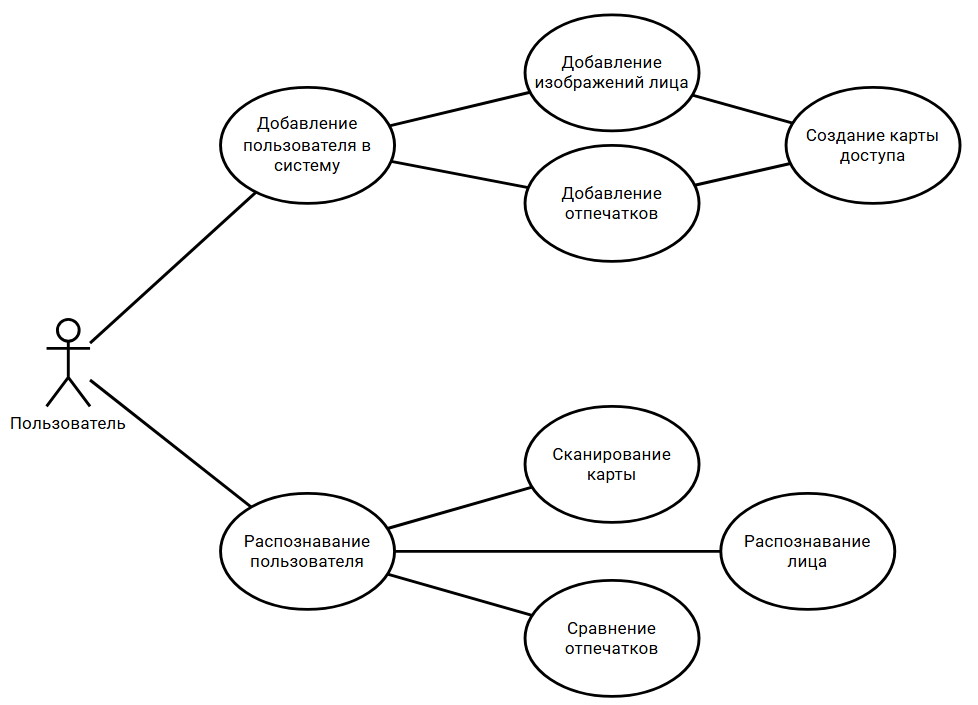
\includegraphics[width=1\linewidth]{images/UML}
	\caption{Диаграмма прецедентов}
	\label{fig:uml}
\end{figure}

\paragraph{Сценарий использования «Добавление изображений лица»}

Заинтересованные лица и их требования: пользователь желает добавить изображения лица в систему.

Предусловие: программа запущена, выбран режим «Добавить в систему».

Постусловие: программа сохраняет изображения лица пользователя  в систему.

Основной успешный сценарий:
\begin{enumerate}
	\item Пользователь нажимает на кнопку «Добавить в систему».
	\item Программа открывает диалоговое окно с указаниями для пользователя.
	\item Пользователь закрывает диалоговое окно.
	\item Программа запускает сканирования лица пользователя.
	\item Пользователь выполняет указания программы.
	\item Программа сохраняет изображения пользователя для дальнейшей обработки.
	\item Программа открывает диалоговое окно с результатом работы.
	\item Пользователь закрывает диалоговое окно и завершает сканирование лица.
\end{enumerate}

\paragraph{Сценарий использования «Добавление отпечатков»}

Заинтересованные лица и их требования: пользователь желает добавить изображения отпечатка в систему.

Предусловие: программа запущена, выбран режим «Добавить в систему», изображения лица добавлены.

Постусловие: программа сохраняет изображения отпечатка пользователя в систему.

Основной успешный сценарий:
\begin{enumerate}
	\item Пользователь нажимает на кнопку «Добавить в систему».
	\item Программа открывает диалоговое окно выбора файла.
	\item Пользователь выбирает файл в формате .jpg, содержащий изображение отпечатка пальца.
	\item Программа запускает обучение нейронной сети на основе изображения отпечатка.
	\item Программа сохраняет модель нейронной сети для дальнейшей работы.
\end{enumerate}

\paragraph{Сценарий использования «Создание карты доступа»}

Заинтересованные лица и их требования: пользователь желает создать карту для доступа в систему.

Предусловие: программа запущена, выбран режим «Добавить в систему», изображения лица и отпечатка добавлены.

Постусловие: программа создает карту доступа в систему.

Основной успешный сценарий:
\begin{enumerate}
	\item Пользователь нажимает на кнопку «Добавить в систему».
	\item Программа запускает создание карты доступа.
	\item Программа сохраняет карту доступа в систему.
\end{enumerate}

\paragraph{Сценарий использования «Сканирование карты»}

Заинтересованные лица и их требования: пользователь желает получить доступ в систему.

Предусловие: программа запущена, выбран режим «Распознавание пользователя».

Постусловие: программа переходит к распознаванию лица.

Основной успешный сценарий:
\begin{enumerate}
	\item Пользователь нажимает на кнопку «Распознавание пользователя».
	\item Программа открывает диалоговое окно с указаниями для пользователя.
	\item Пользователь закрывает диалоговое окно.
	\item Пользователь выполняет указания программы.
	\item Программа запускает сканирования карты пользователя.
	\item Программа получает данные с карты для дальнейшего распознавания.
\end{enumerate}

\paragraph{Сценарий использования «Распознавание лица»}

Заинтересованные лица и их требования: пользователь желает получить доступ в систему.

Предусловие: программа запущена, выбран режим «Распознавание пользователя», карта доступа распознана.

Постусловие: программа переходит к сравнению отпечатка.

Основной успешный сценарий:
\begin{enumerate}
	\item Пользователь нажимает на кнопку «Распознавание пользователя».
	\item Программа открывает диалоговое окно с указаниями для пользователя.
	\item Пользователь закрывает диалоговое окно.
	\item Пользователь выполняет указания программы.
	\item Программа запускает сканирования карты пользователя.
	\item Программа получает данные с карты для дальнейшего распознавания.
\end{enumerate}

\paragraph{Сценарий использования «Сравнение отпечатков»}

Заинтересованные лица и их требования: пользователь желает получить доступ в систему.

Предусловие: программа запущена, выбран режим «Распознавание пользователя», карта доступа и лицо распознаны.

Постусловие: программа выдает результат распознавания.

Основной успешный сценарий:
\begin{enumerate}
	\item Пользователь нажимает на кнопку «Распознавание пользователя».
	\item Программа открывает диалоговое окно с указаниями для пользователя.
	\item Пользователь закрывает диалоговое окно.
	\item Пользователь выполняет указания программы.
	\item Программа запускает сканирования карты пользователя.
	\item Программа получает данные с карты для дальнейшего распознавания.
\end{enumerate}


\subsubsection{Требования пользователя к интерфейсу приложения}

 Приложение должно иметь следующие экраны:
 
 \begin{enumerate}
 	\item Экран «Идентификация». Основной экран, реализующий
 	функционал распознавания пользователя на основе изображений лица и отпечатка пальца.
 	\item Экран «Добавление в систему». Экран, позволяющий добавлять пользователя в систему, путём сохранения изображений лица и отпечатков пальца с генерацией карты доступа.
 \end{enumerate}


\subsubsection{Нефункциональные требования к программной системе}

\paragraph {Требования к надежности}

Программная система должна обеспечивать стабильную работу в различных условиях эксплуатации. В процессе работы приложения могут возникнуть следующие аварийные ситуации:
\begin{enumerate}
	\item отсутствие подключения к камере для получения изображений;
	\item ошибка доступа к файлам изображения;
\end{enumerate}

Для предотвращения аварийных ситуаций программа должна корректно обрабатывать исключения при работе с файлами, предоставляя пользователям информативные сообщения об ошибках. В случае проблем с отсутствием прав доступа к директории сохранения файлов, полученных в результате работы программы, программа должна открывать диалоговое окно с выбором другой директории.

\paragraph {Требования к программному обеспечению}

Для запуска и работы программы требуется компьютер под управлени
ем операционной системы Windows 10 или Windows 11. При использовании
графических адаптеров NVIDIA с поддержкой технологии CUDA для уско
рения обучения нейронной сети необходима последняя версия драйверов со
ответствующего адаптера, а также программы CUDA Toolkit и cuDNN

\paragraph {Требования к аппаратному обеспечению}

Для корректной работы программного продукта, реализующего распознавание лиц, отпечатков пальцев и идентификаторов карт доступа, требуется центральный процессор с количеством ядер от 6 и выше и тактовой частотой не менее 2.4 ГГц. Объём оперативной памяти должен составлять не менее 8 ГБ.

Для захвата изображений лиц обязательно наличие веб-камеры с разрешением не менее 1280×720 пикселей. Камера должна обеспечивать чёткое изображение при нормальном освещении.

Для сохранения изображений отпечатков пальцев может потребоваться сканер с разрешением не менее 500 dpi, совместимый с операционной системой и поддерживаемый программной частью.

\subsection{Требования к оформлению документации}

Разработка программной документации и программного изделия должна производиться согласно ГОСТ 19.102-77 и ГОСТ 34.601-90. Единая система программной документации.

Программная документация должна включать в себя:
\begin{itemize}
	\item анализ предметной области;
	\item техническое задания;
	\item технический проект;
	\item рабочий проект.
\end{itemize}
\section{Технический проект}
\subsection{Общая характеристика организации решения задачи}

Необходимо спроектировать и разработать систему, которая должна выполнять распознавание на основе изображений лиц и отпечатков пальцев с использованием карт пропуска.

Система представляет собой программу, позволяющую пользователю выполнять распознавание лиц и отпечатков пальцев и сканирование карты пропуска для авторизации. Интерфейс включает в себя окно, отображающее видеопоток с камеры и результаты распознавания лица или отпечатка пальца и карты пропуска. Программа автоматически определяет лицо, отпечаток пальца или карту пропуска в кадре, сопоставляет данные и отображает результаты выполнения программы на экране. 

\subsection{Обоснование выбора технологии проектирования}

Используемые для создания интеллектуальной системы языки программирования и технологии соответствуют современным практикам разработки, обеспечивают высокую производительность и отказоустойчивость системы.

\subsubsection{Описание используемых технологий и языков программирования}

В процессе разработки программы используется язык программирования Python, а также сторонние библиотеки OpenCV, PyTorch, NumPy, tkinter и Python Imaging Library.

\subsubsection{Язык программирования Python}

Язык программирования Python представляет собой высокоуровневый язык общего назначения, отличающийся лаконичным синтаксисом и высокой читаемостью кода. Python обеспечивает возможность реализации объектно-ориентированного, функционального и процедурного стилей программирования. Он обладает мощной стандартной библиотекой, которая охватывает множество областей применения — от работы с файлами и сетями до многопоточности и регулярных выражений. Python широко используется в научных вычислениях, благодаря таким библиотекам как NumPy, SciPy, Pandas и Matplotlib. В области машинного обучения и нейросетей Python является наилучшим языком программирования, благодаря таким инструментам как PyTorch, TensorFlow и Scikit-learn. Кроме того, язык поддерживается большим сообществом, что облегчает поиск решений и развитие проектов.

\subsubsection{Библиотека OpenCV}

OpenCV представляет собой мощную библиотеку компьютерного зрения и обработки изображений, предназначенную для выполнения широкого спектра задач, связанных с анализом изображений и видео. Она предоставляет высокоуровневые и низкоуровневые средства для работы с изображениями, включая функции для обработки, фильтрации, распозна-вания объектов и анализа движения. Основное преимущество OpenCV заключается в её высокой производительности, гибкости и поддержке широкого спектра алгоритмов компьютерного зрения. Благодаря интеграции с языком Python, OpenCV позволяет быстро разрабатывать приложения, связанные с обработкой изображений и видео, и является популярным инструментом как для учебных, так и для полноценных исследовательских и промышленных проектов.

\subsubsection{Библиотека PyTorch}

PyTorch — это современная библиотека машинного и глубокого обучения, предназначенная для создания и обучения нейронных сетей. Она предоставляет интуитивно понятные инструменты для работы с тензорами, автоматического дифференцирования и построения моделей. Одним из ключевых преимуществ PyTorch является использование динамической вычислительной графики, что делает разработку и отладку нейросетей более гибкой и наглядной. Библиотека поддерживает ускорение вычислений с помощью графических процессоров (GPU), что существенно повышает производительность при обучении моделей. Благодаря тесной интеграции с Python, а также множеству встроенных модулей и готовых архитектур, PyTorch широко применяется в задачах компьютерного зрения, обработки естественного языка, биометрии и других областях искусственного интеллекта.

\subsubsection{Библиотека NumPy}

NumPy представляет собой фундаментальную библиотеку для численных вычислений в Python, обеспечивающую поддержку многомерных массивов и высокоуровневых математических операций над ними. Благодаря высокоэффективным операциям с массивами и встроенным линейным алгебраическим методам, NumPy позволяет обрабатывать изображения больших размеров с минимальными затратами ресурсов, что делает её незаменимой в задачах, связанных с сжатием, декомпрессией и преобразованием графических данных.

\subsubsection{Библиотека tkinter}

Для построения графического интерфейса в проекте выбрана библиотека tkinter, которая является частью стандартной поставки Python и представляет собой обёртку над библиотекой Tcl/Tk. Этот выбор объясняется рядом технологических и практических преимуществ:
\begin{enumerate}
	\item Отсутствие необходимости в установке сторонних зависимостей делает tkinter особенно удобным для использования в проектах с упрощённым процессом развёртывания. Пользователь может сразу запустить приложение без дополнительных установок, что критично в условиях учебной и демонстрационной среды.
	\item Простота проектирования интерфейса позволяет легко создавать окна, формы, кнопки, меню, вкладки и другие элементы без необходимости изучения сложных графических фреймворков. Это способствует быстрому созданию прототипов и конечных версий интерфейса.
	\item Полная кроссплатформенность интерфейса гарантирует его одинаковое отображение и поведение на всех операционных системах, что избавляет разработчика от необходимости писать отдельные реализации под разные платформы.
	\item Наличие компонентов высокого уровня, таких как текстовые поля, выпадающие списки, кнопки, панели и таблицы, даёт возможность создать функциональный и интуитивно понятный интерфейс для работы с данными.
	\item Возможность динамического обновления интерфейса обеспечивает удобную визуализацию изменений.
\end{enumerate}

tkinter полностью удовлетворяет требованиям к простому, лёгкому в использовании, но функциональному графическому интерфейсу, особенно в условиях ограниченного времени и ресурсов.	

\subsubsection{Python Imaging Library}

Python Imaging Library, сокращенно PIL — это библиотека для работы с растровыми изображениями, обеспечивающая поддержку различных форматов, таких как JPEG, PNG, BMP и других. PIL предоставляет широкий набор функций для загрузки, сохранения, обработки и преобразования изображений, что упрощает различные взаимодействия с файлами изображений, такие как сохранение и загрузка изображений, поэтому она является удобным инструментом для предварительной и финальной обработки графических данных.



\subsection{Архитектура программной системы}

Точкой входа в программу является модуль main.py, в котором создаётся и запускается экземпляр класса App, реализующего основной графический интерфейс приложения. Архитектура программы ориентирована на модульность и разделение ответственности, что облегчает поддержку, тестирование и возможное расширение проекта.

Архитектура приложения состоит из следующих ключевых модулей:
\begin{enumerate}
	\item programm.py — стартовый модуль, в котором производится инициализация пользовательского интерфейса. Здесь создаётся объект MainWindow, который затем запускается методом mainloop(). Содержит в себе код основных классов приложения(App и LoadingScreen).
	
	\item func.py — содержит функции детекции лиц, извлечения эмбеддингов, сравнения лиц и работы с моделями для распознавания. Модуль отвечает за большинство вычислений в системе.
	
	\item model.py — реализует классы FingerprintEncoder и SiameseNetwork, предназначенные для обработки изображений отпечатков пальцев. Класс FingerprintEncoder — это нейронная сеть, основанная на архитектуре ResNet-18, модифицированная для извлечения эмбеддингов изображений отпечатков пальцев. Класс SiameseNetwork — это основная модель, использующая подход сиамской нейронной сети, где сравниваются два изображения. Эта сеть обучается таким образом, чтобы оценить, являются ли два изображения схожими или нет.
	
	\item dataset.py — создает пользовательскую выборку для обучения модели с использованием пар изображений отпечатков пальцев. Модуль создает как положительные, так и отрицательные пары изображений, которые используются для обучения сиамской сети.
	
	\item train.py — представляет собой процесс обучения модели для сравнения отпечатков пальцев с использованием сиамской нейронной сети и последующего сохранения обученной модели.
	
	\item fp.py — содержит реализацию обработки векторных представлений в классе Fingerprints. Класс Fingerprints используется для сравнения двух изображений отпечатков пальцев и оценки их схожести. Система использует модель Siamese Network, обученную для нахождения эмбеддингов (векторных представлений) изображений отпечатков пальцев, и затем вычисляет схожесть между этими эмбеддингами с использованием косинусного сходства.
	
	\item save\_face.py — захват изображений лиц с камеры и их сохранения в определенную директорию для дальнейшей тренировки модели распознавания лиц.
	
	\item embedding\_create.py — используется для извлечения векторных представлений лиц из изображений и сохранения их для последующего распознавания личности по лицу.
	
\end{enumerate}

Компоненты программы взаимодействуют следующим образом:
\begin{enumerate}
	\item Интерфейс (класс App из файла programm.py) получает данные пользователя, например, запрос на распознавание лица или отпечатка пальца, и передаёт их на обработку соответствующим функциям.
	
	\item Модуль func.py обрабатывает эти команды: выполняет детекцию лиц, извлекает эмбеддинги с помощью нейросетевых моделей, сравнивает их с ранее сохранёнными представлениями и возвращает результат.
	
	\item Результаты распознавания отображаются в пользовательском интерфейсе. При этом данные могут быть изменены или обновлены в зависимости от действий пользователя.
	
	\item Модули save\_face.py и embedding\_create.py используются для подготовки базы данных лиц: save\_face.py захватывает изображения с камеры, а embedding\_create.py извлекает и сохраняет их эмбеддинги.
	
	\item Для распознавания отпечатков пальцев используется модель, реализованная в файле model.py и обученная с помощью модуля train.py. Сравнение векторных представлений отпечатков выполняется в модуле fp.py на основе косинусного расстояния.
	
	\item Все изображения и векторные представления хранятся в структуре каталогов database/, что позволяет системе работать автономно, без внешней базы данных.
\end{enumerate}

Между компонентами поддерживается минимальная необходимая связь: графический интерфейс не содержит логики обработки выражений, а логика ядра независима от визуального представления. Это упрощает поддержку, тестирование и адаптацию системы для различных платформ.

Архитектура гибкая, расширяемая и легко масштабируемая. Возможность добавления новых типов команд или подключения внешних источников данных или API без необходимости переписывания основной логики делает систему адаптируемой к разнообразным задачам.

\ifПрактика{}\else{
   \section{Рабочий проект}
\subsection{Классы, используемые при разработке сайта}

Можно выделить следующий список классов и их методов, использованных при разработке web-приложения (таблица \ref{class:table}). Пример таблицы с уменьшенным межстрочным интервалом.

\renewcommand{\arraystretch}{0.8} % уменьшение расстояний до сетки таблицы
\begin{xltabular}{\textwidth}{|X|p{2.5cm}|>{\setlength{\baselineskip}{0.7\baselineskip}}p{4.85cm}|>{\setlength{\baselineskip}{0.7\baselineskip}}p{4.85cm}|}
\caption{Описание классов Bitrix, используемых в приложении\label{class:table}}\\
\hline \centrow \setlength{\baselineskip}{0.7\baselineskip} Название класса & \centrow \setlength{\baselineskip}{0.7\baselineskip} Модуль, к которому относится класс & \centrow Описание класса & \centrow Методы \\
\hline \centrow 1 & \centrow 2 & \centrow 3 & \centrow 4\\ \hline
\endfirsthead
\caption*{Продолжение таблицы \ref{class:table}}\\
\hline \centrow 1 & \centrow 2 & \centrow 3 & \centrow 4\\ \hline
\finishhead
CMain & Главный модуль & CMain – главный класс страницы web-приложения. После одного из этапов по загрузке страницы в сценарии становится доступным инициализированный системой объект данного класса с именем \$APPLICATION & void ShowTitle(string property\_code = «title», bool strip\_tags = true)
Выводит заголовок страницы
void SetTitle(string title)
Устанавливает заголовок страницы

void ShowCSS(bool external = true, bool XhtmlStyle = true)
Выводит таблицу стилей CSS страницы\\
\hline CFile & Главный модуль & CFile – Класс для работы с файлами и изображениями & array GetFileArray (int file\_id)
Метод возвращает массив, содержащий описание файла (путь к файлу, имя файла, размер) с идентификатором file\_id
\end{xltabular}
\renewcommand{\arraystretch}{1.0} % восстановление сетки

\subsection{Модульное тестирование разработанного web-сайта}

Модульный тест для класса User из модели данных представлен на рисунке \ref{unitUser:image}.

\begin{figure}[ht]
\begin{lstlisting}[language=Python]
from django.test import TestCase
from .models import *
User = get_user_model()


class ShpoTestCases(TestCase):

    def setUp(self) -> None:
        self.user = User.objects.create(username='testtestovich', password='testtestovich', first_name='Sad', last_name='')

    def test_2(self):

        self.assertEqual(self.user.first_name, 'Sad')
        self.assertEqual(self.user.last_name, 'Cat')
        print((self.user))
        print((self.user.first_name))
        print((self.user.last_name))
\end{lstlisting}  
\caption{Модульный тест класса User}
\label{unitUser:image}
\end{figure}

\subsection{Системное тестирование разработанного web-сайта}

На рисунке \ref{main:image} представлена главная страница сайта «Русатом – Аддитивные технологии».
\newpage % при необходимости можно переносить рисунок на новую страницу
\begin{figure}[H] % H - рисунок обязательно здесь, или переносится, оставляя пустоту
\center{\includegraphics[width=1\linewidth]{main1}}
\center{\includegraphics[width=1\linewidth]{main2}}
\center{\includegraphics[width=1\linewidth]{main3}}
\caption{Главная страница сайта «Русатом – Аддитивные технологии»}
\label{main:image}
\end{figure}

На рисунке \ref{menu:image} представлен динамический вывод заголовков, включающий в себя искомые фразы при поиске фраз.

\begin{figure}[ht]
\center{\includegraphics[width=1\linewidth]{menu}}
\caption{Динамический вывод заголовков}
\label{menu:image}
\end{figure}

На рисунке \ref{enter:image} представлен ввод данных для публикации новости.

\begin{figure}[ht]
\center{\includegraphics[width=1\linewidth]{enter}}
\caption{Ввод данных для публикации очень-очень длинной, интересной и полезной новости}
\label{enter:image}
\end{figure}

   \section*{ЗАКЛЮЧЕНИЕ}
\addcontentsline{toc}{section}{ЗАКЛЮЧЕНИЕ}

Преимущества аддитивных технологий заключается в разнообразии процессов, позволяющих применять их в различных областях производства. Существенным ограничением же является и экономическая составляющая, которая не позволит внедрить аддитивное производство повсеместно.
  
Компании, видя, как развиваются информационные технологии, пытаются использовать их выгодно для своего бизнеса, запуская свой сайт для того, чтобы заявить о своем существовании, проинформировать потенциального клиента об услугах или продуктах, которые предоставляет. 
Для продвижения компании «Русатом – Аддитивные технологии» был разработан веб-сайт на основе системы «1С-Битрикс: Управление сайтом».

Основные результаты работы:

\begin{enumerate}
\item Проведен анализ предметной области. Выявлена необходимость использовать 1С-Битрикс.
\item Разработана концептуальная модель web-сайта. Разработана модель данных системы. Определены требования к системе.
\item Осуществлено проектирование web-сайта. Разработана архитектура серверной части. Разработан пользовательский интерфейс web-сайта.
\item Реализован и протестирован web-сайт. Проведено модульное и системное тестирование.
\end{enumerate}

Все требования, объявленные в техническом задании, были полностью реализованы, все задачи, поставленные в начале разработки проекта, были также решены.

Готовый рабочий проект представлен адаптивной версткой сайта. Сайт находится в публичном доступе, поскольку опубликован в сети Интернет.  

}\fi
\addcontentsline{toc}{section}{СПИСОК ИСПОЛЬЗОВАННЫХ ИСТОЧНИКОВ}

\begin{thebibliography}{9}

    \bibitem{sis} Большаков И. А. Системы распознавания лиц – принцип работы и сферы применения / И. А. Большаков, С. А. Микаева. – Текст : непосредственный // Науносфера. – 2022. – № 9-2. – С. 95–98.
    
    \bibitem{abdulaev} Абдуллаев А. И. Распознавание лиц по изображению лица / А. И. Абдуллаев. – Текст : непосредственный // Мировая наука. – 2021. – № 4 (49). – С. 44–47.
    
    \bibitem{moscow} Кандидата наук Ермошина задержали как вора из-за ошибки распознавания лиц [Электронный ресурс] // Московский комсомолец. – 2021. – 19 октября. – URL: https://www.mk.ru/incident/2021/10/19/kandidata-nauk-ermoshina-zaderzhali-kak-vora-izza-oshibki-raspoznavaniya-lic.html? utm\_source=yxnews\&utm\_medium=desktop (дата обращения: 03.05.2025).
    
     \bibitem{four} Байкенов Б. С. Сравнительный анализ методов распознавания объектов / Б. С. Байкенов, Р. С. Тынчеров, А. Р. Фазылова. – Текст : непосредственный // Вестник Казахской академии транспорта и коммуникаций им. М. Тынышпаева. – 2019. – № 1 (108). – С. 185–191.
     
     \bibitem{history} Ветров С. В. История развития систем распознавания лиц / С. В. Ветров. – Текст : непосредственный // Наука и образование: актуальные исследования и разработки : материалы IV Всероссийской научно-практической конференции / отв. ред. А. В. Лесков. – Чита : Забайкальский государственный университет, 2021. – С. 23–29.
     
     \bibitem{six} Джеймс, Р. UML 2.0. Объектно-ориентированное моделирование и
     разработка / Р. Джеймс, Б. Майкл.– 2-е изд.– Санкт-Петербург : Питер, 2021.– 542 с.– ISBN 978-5-4461-9428-5.– Текст : непосредственный. 
     
     \bibitem{seven} Биэль, М. RESTful API Design / М. Биэль.– University Press, 2016.
     300 с.– ISBN 978-1-5147-3516-9.– Текст : непосредственный.
     
     \bibitem{eight} Аттуи, А. Real-Time and Multi-Agent Systems / А. Аттуи.– Springer
     Science \& Business Media, 2000.– 496 с.– ISBN 978-1-85233-252-5.– Текст :
     непосредственный.
     
     
     \bibitem{eleven} Буч, Г. Введение в UML от создателей языка / Г. Буч, И. Якобсон,
     Д. Рамбо.– Москва : ДМК Пресс, 2015.– 498 с.– ISBN 978-5-457-43379-3.
     Текст : непосредственный.
     
     
     \bibitem{twelve} Мандел, Т. Разработка пользовательского интерфейса / Т. Мандел.– ДМК Пресс, 2019.– 420 с.– ISBN 978-5-04-195060-6.– Текст : непосредственный.
     
     \bibitem{twelve} 5.	Мартин, Р. Чистая архитектура. Искусство разработки про-граммного обеспечения / Р. Мартин; пер. с англ. А. Кисилева. – Санкт-Петербург: Питер, 2018. – 351 с. – ISBN 978-5-4461-0772-8. – Текст: непо-средственный.
     
    
\end{thebibliography}

\ifВКР{\appendix{Представление графического материала}

Графический материал, выполненный на отдельных листах,
изображен на рисунках А.1--А.\arabic{числоПлакатов}.
\setcounter{числоПлакатов}{0}

\renewcommand{\thefigure}{А.\arabic{figure}} % шаблон номера для плакатов

\begin{landscape}

\begin{плакат}
    
\includegraphics[width=0.82\linewidth]{плакат1.png}
    \заголовок{Сведения о ВКРБ}
    \label{pl1:image}      
\end{плакат}

\begin{плакат}
    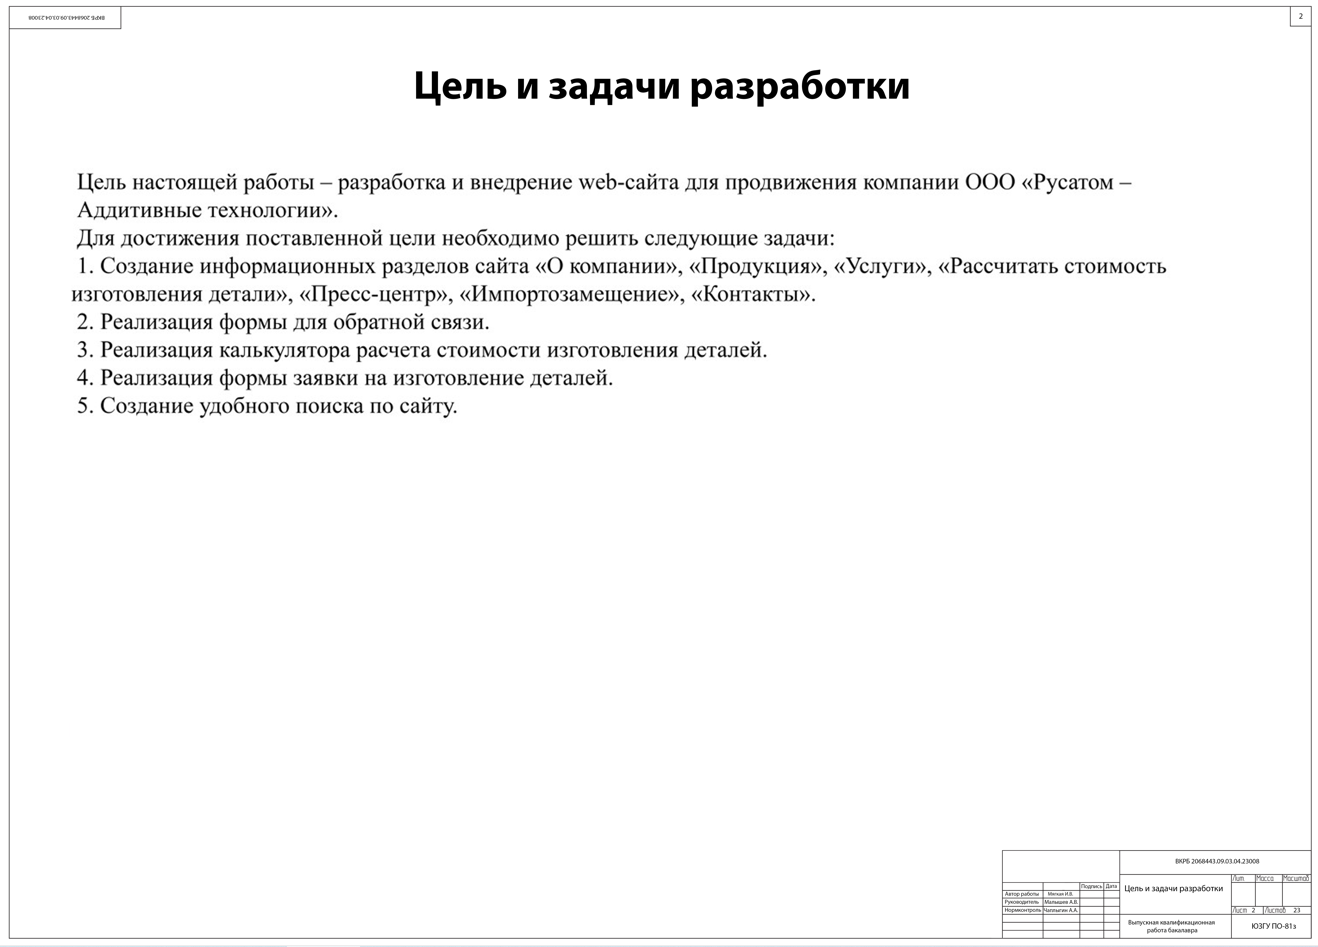
\includegraphics[width=0.82\linewidth]{плакат2.png}
    \заголовок{Цель и задачи разработки}
    \label{pl2:image}      
\end{плакат}

\begin{плакат}
    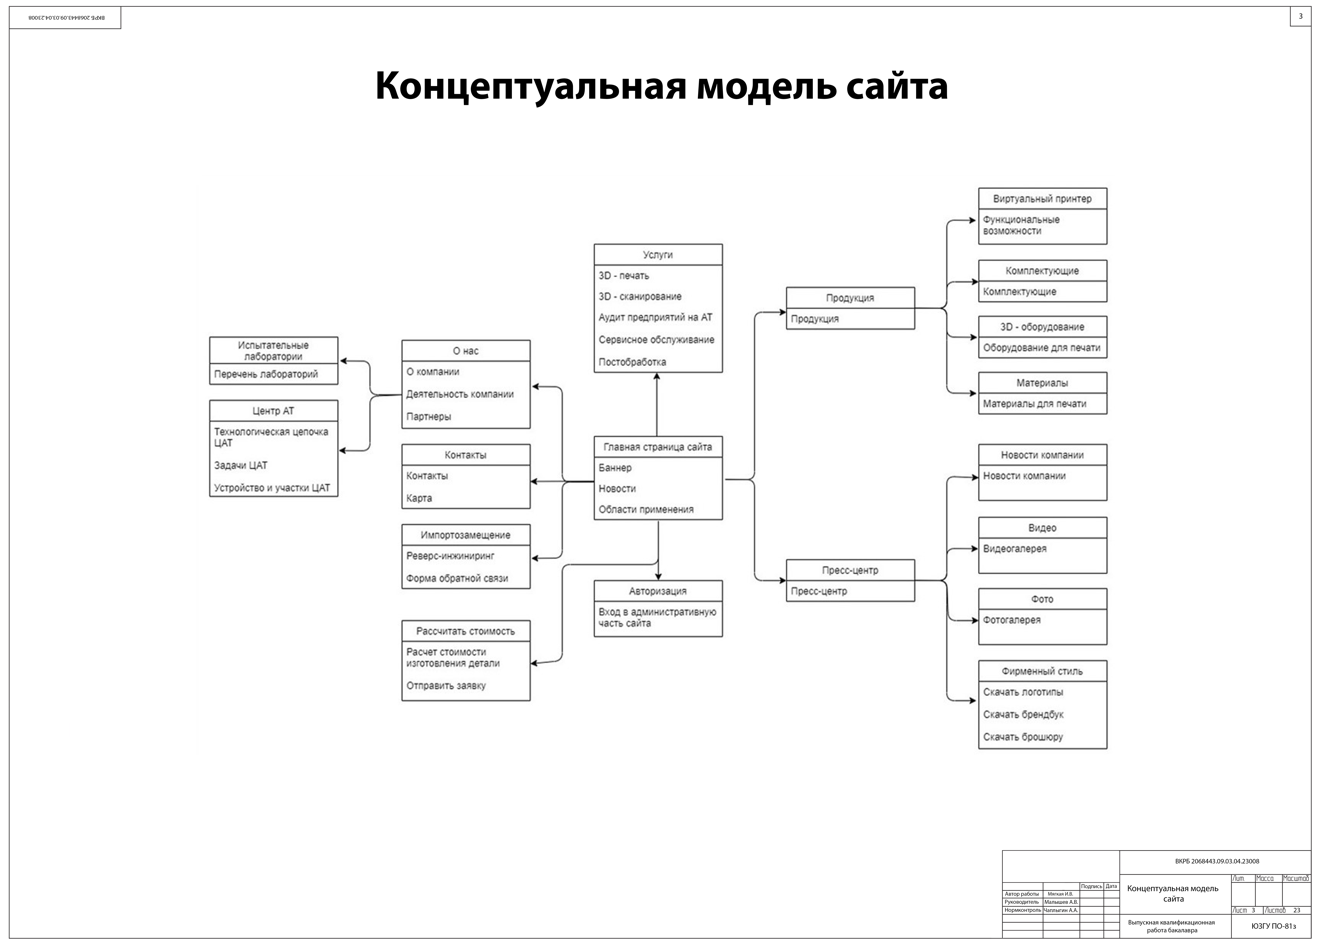
\includegraphics[width=0.82\linewidth]{плакат3.png}
    \заголовок{Концептуальная модель сайта}
    \label{pl3:image}      
\end{плакат}

\begin{плакат}
    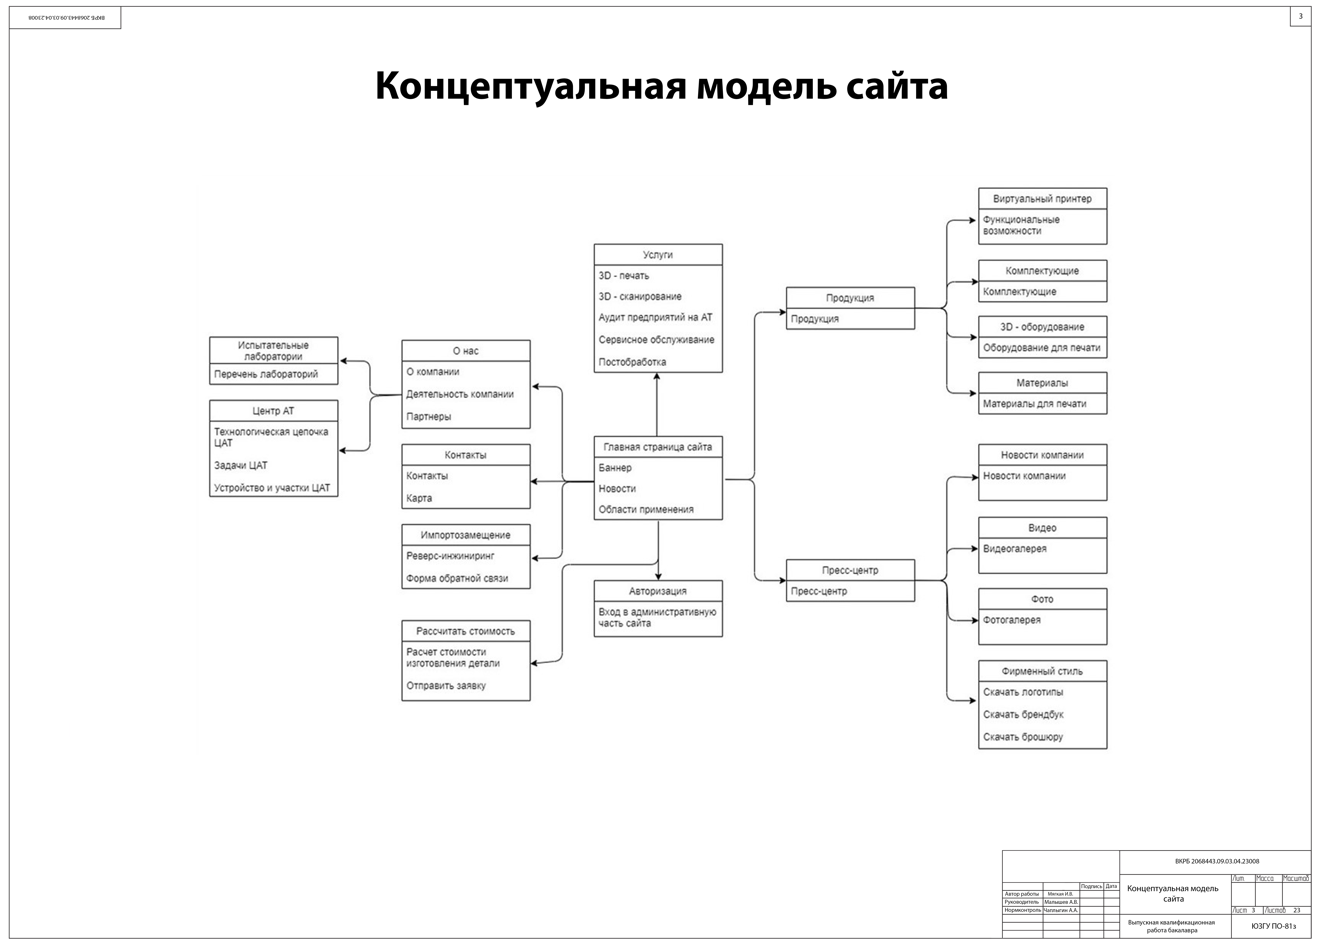
\includegraphics[width=0.82\linewidth]{плакат3.png}
    \заголовок{Еще плакат}
    \label{pl4:image}      
\end{плакат}

\end{landscape}
}\fi
\ifПрактика{}\else{\appendix{Фрагменты исходного кода программы}

main.tex
\lstinputlisting[language=Tex, frame=none]{main.tex}

ТехПроект.tex
\lstinputlisting[language=Tex, frame=none]{ТехПроект.tex}

\ifВКР{
\newpage
\addcontentsline{toc}{section}{На отдельных листах (CD-RW в прикрепленном конверте)}
\noindent
\begin{tabular}{p{5.8cm}C{4.8cm}C{4.8cm}}
   Автор ВКР & \lhrulefill{\fill} & \fillcenter\Автор \\
            \setarstrut{\footnotesize}
           & \footnotesize{(подпись, дата)} & \\
            \restorearstrut
   Руководитель ВКР & \lhrulefill{\fill} & \fillcenter\Руководитель \\
            \setarstrut{\footnotesize}
           & \footnotesize{(подпись, дата)} & \\
            \restorearstrut
   Нормоконтроль & \lhrulefill{\fill} & \fillcenter\Нормоконтроль \\
            \setarstrut{\footnotesize}
           & \footnotesize{(подпись, дата)} & \\
            \restorearstrut
\end{tabular}
\vskip 2cm
\begin{center}
\textbf{Место для диска}
\end{center}
}\fi
}\fi
\end{document}
